
\chapter{Was ist Physik?}
\label{ch:wasistphysik}

\begin{aquote}{Albert Einstein}
    All unsere Wissenschaft ist, gemessen an der Wirklichkeit, primitiv und kindlich - und doch ist sie unser kostbarstes Gut. 
\end{aquote}

Die Physik ist eine Naturwissenschaft\footnote{u.a. Physik, Chemie, Biologie, Geologie} und versucht somit die Vorgänge in der Natur zu beschreiben und zu messen. Sie gehört wie auch die Mathematik zu den ``exakten Wissenschaften''. Die Arbeitsweise der Physik besteht im Zusammenspiel von theoretischer Modellbildung und experimentellen Methoden.
\begin{marginfigure}
	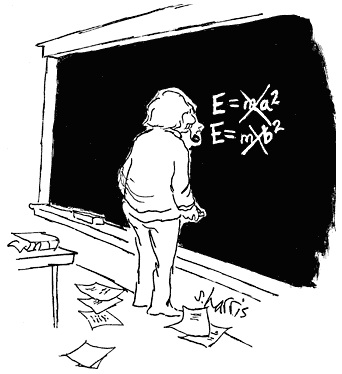
\includegraphics[width=0.7\textwidth]{Bilder/einstein.jpg}
	\label{fig:einsteinfig}
\end{marginfigure} 

Die Physik versucht, die Natur zu beschreiben, nicht zu erklären. Dies ist ein wesentlicher Unterschied, der insbesondere Physik und Philosophie voneinander trennt. Die Physik hinterfragt die Natur nicht, sie verwendet die gegebenen Tatsachen, versucht sie mit mathematischen Mitteln darzustellen und dann daraus mittels den Methoden der Logik weitere, beobachtbare Tatsachen abzuleiten; also Voraussagen zu treffen, wie sich ein System unter gegebenen Bedingungen verhalten wird. Andererseits muss das mathematische Modell auch fähig sein, bereits bekannte
Phänomene hinreichend gut (d.h. innerhalb der unvermeidbaren Messtoleranz) beschreiben zu
können. Ein solches mathematisches Modell, welches diese beiden Bedingungen erfüllt, bezeichnet
man als Theorie.

\section{Womit beschäftigt sich Physik?}
\begin{marginfigure}
    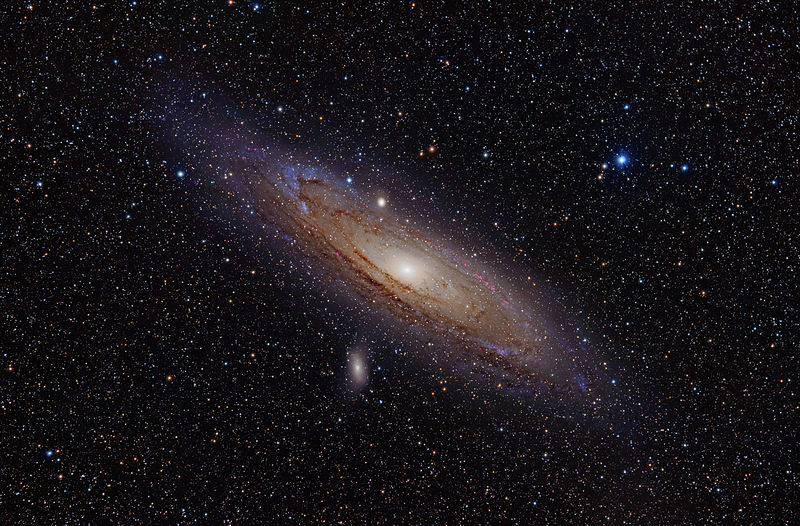
\includegraphics[width=0.7\textwidth]{Bilder/andromeda.jpg}
\end{marginfigure}

Die Physik beschäftigt sich mit Bewegungen von Objekten, vom kleinsten Elementarteilchen bis hin zu den Galaxien. Sie untersucht die in der Natur wirksamen Kräfte, wie zum Beispiel die Gravitationskraft zwischen Massen. Sie beschreibt Vorgänge auf der Erde, auf der Sonne und im gesamten Universum. In der modernen Physik konnten alle unterschiedlichen Teilgebiete zu bislang zwei grundsätzlich verschiedenen Theorien zusammengefasst werden; dem ``Standartmodell der Teilchenphysik'' und der ``Allgemeinen Relativitätstheorie''. 
\begin{marginfigure}
    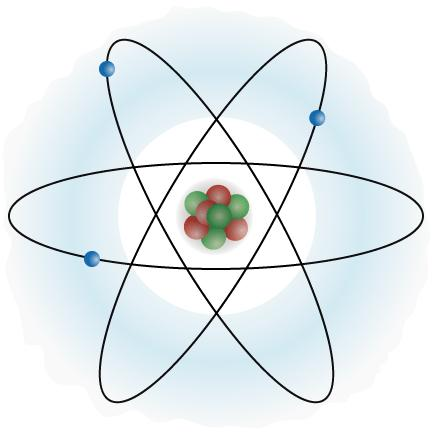
\includegraphics[width=0.7\textwidth]{Bilder/atom.jpg}
\end{marginfigure}
Bis heute haben die Physiker jedoch keinen Weg gefunden, diese beiden grossen Gebiete unter einen Hut zu bringen. Dies ist eines der ganz grossen Ziele der heutigen Physik. Diese Vereinheitlichung aller bekannten Kräfte wird auch ``Weltformel''\footnote{engl. ``Theory of Everything''} genannt.


\section{Weshalb lernen wir Physik?}
\begin{marginfigure}
    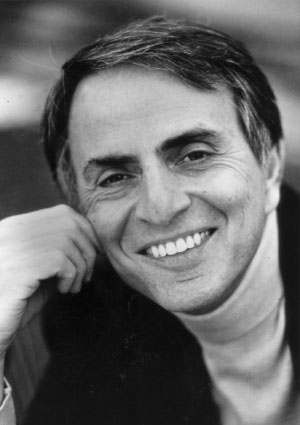
\includegraphics[width=0.7\textwidth]{Bilder/sagan.jpg}
	\label{fig:sagan}
\end{marginfigure} 
\begin{aquote}{Carl Sagan, 1989}
	Wir leben in einer Gesellschaft, die in hohem Masse von Wissenschaft und Technik abhängig ist, in der allerdings kaum jemand etwas über Wissenschaft und Technik weiss. Das ist ein direkter Weg in die Katastrophe.
\end{aquote}
Die Physik ermöglicht uns, die Abläufe in der Natur zu verstehen. Sie bildet die Grundlage der heutigen Technologie und ist für zahlreiche wirtschaftliche und gesellschaftliche Fragen relevant. Die Bedeutung der Physik für die heutige Gesellschaft wird besonders deutlich bei unserer Abhängigkeit von der Technik: Sehr viele der Technologien, die die Welt ständig verändern lassen sich direkt auf wichtige physikalische Forschung zurückführen. Zum Beispiel ermöglichte die Erforschung der Physik der Halbleiter die Entwicklung des ersten Transistors im Jahre 1947.
\begin{marginfigure}
    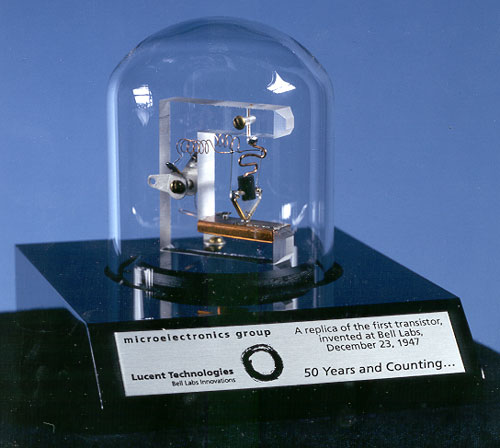
\includegraphics[width=0.7\textwidth]{Bilder/transistor.jpg}
    \label{fig:transistor}
\end{marginfigure} 
Dieses scheinbar simple Stück Technik ist die Schlüsselkomponente in all unserer elektronischen Geräte, inklusive Computer und Smartphone und wird heute als die wichtigste Erfindung in der Geschichte der Menschheit betrachtet. Die Gesetze der Optik, die das Verhalten von Lichtstrahlen beschreiben, führten zu der Entwicklung der optischen Fibernetzwerke, die beginnen, die Welt zu umspannen und näher zusammenzuführen.

Auf einer weniger greifbareren Ebene haben uns die physikalischen Theorien ermöglicht ein grösseres Verständnis des Universums in dem wir leben zu erhalten. Es sind diese Theorien, die uns die tiefgründigsten Beschreibungen von Raum, Zeit, Materie und Energie ermöglichen. Physikalische Theorien erlauben uns die Grundbausteine aller Materie zu verstehen. Dies sind Dinge, die wir nie im alltäglichen Leben erfahren können. Im anderen Extrem beschreiben die Theorien der Kosmologie den Anfang des Universums und sagen uns, wie dieses enden könnte. 
\begin{marginfigure}
    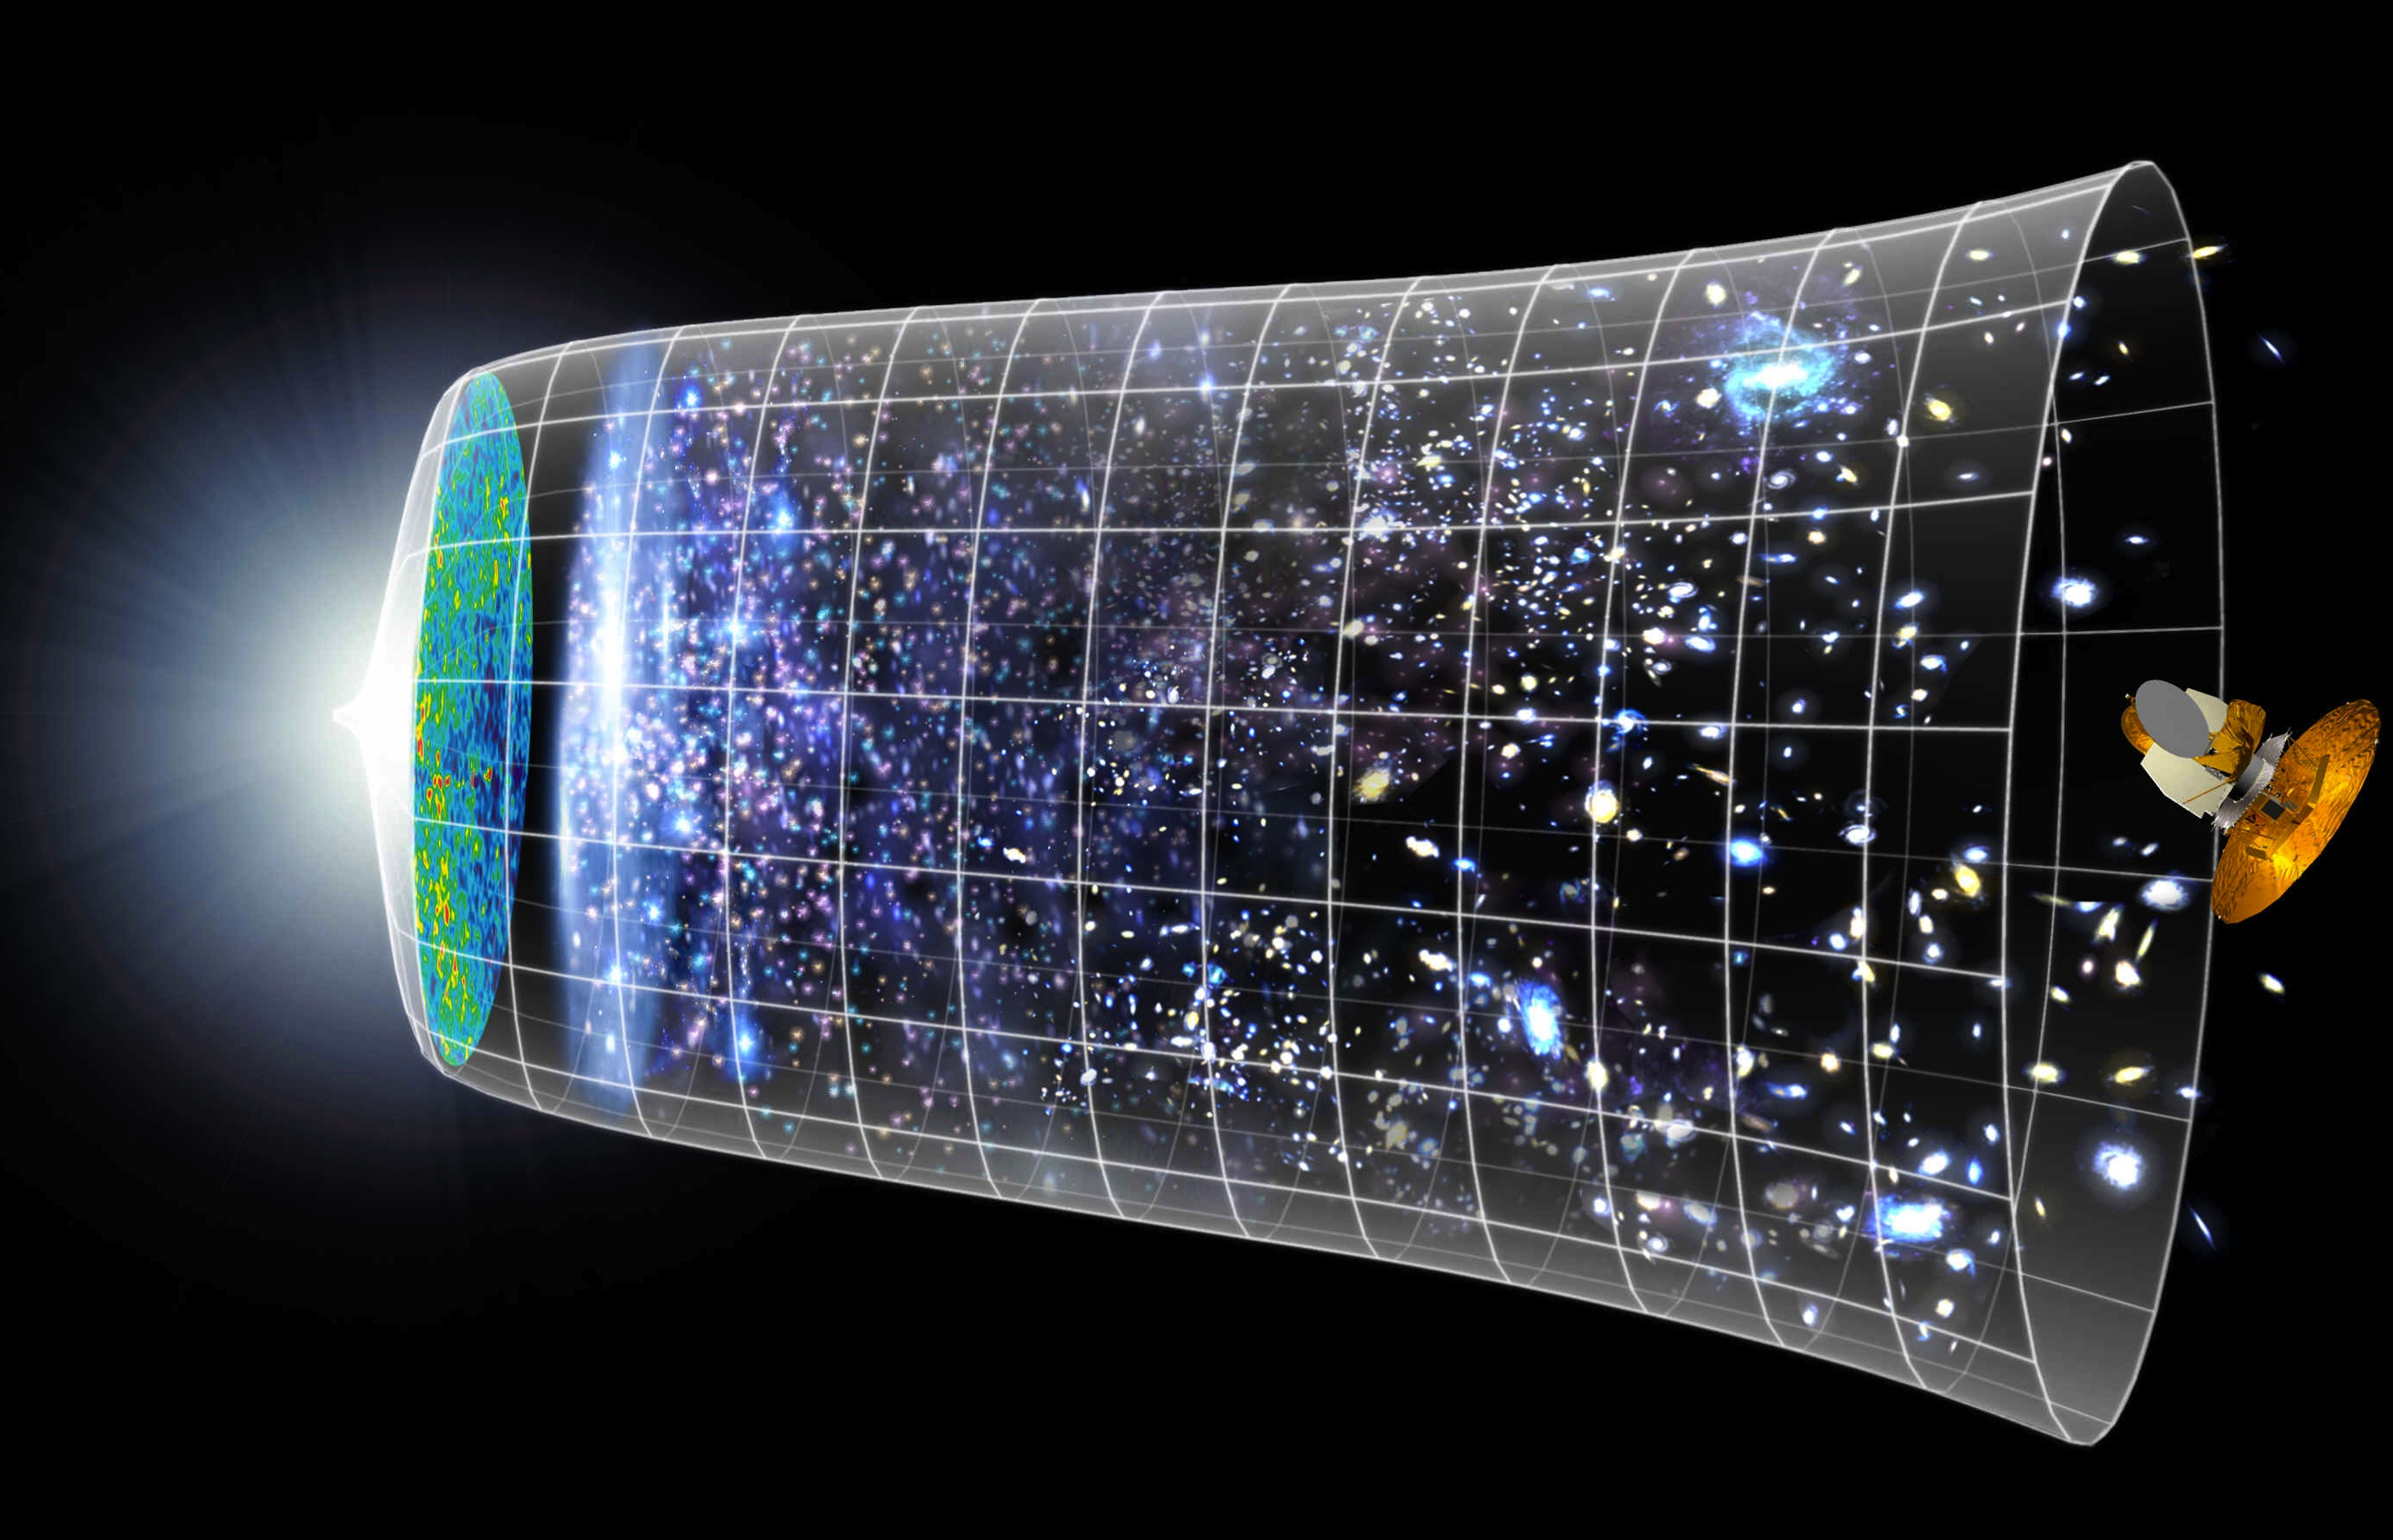
\includegraphics[width=0.7\textwidth]{Bilder/wmap.jpg}
    \label{fig:wmap}
\end{marginfigure} 

\chapter{Grundlagen}
\section{Mathematische Werkzeuge}
\begin{marginfigure}
	
\includegraphics[width=0.7\textwidth]{Bilder/toolbox.jpg}
	\label{fig:toolboxfig}
\end{marginfigure} 
Zu den grundlegenden mathematischen Werkzeugen, die wir im Physikunterricht benötigen werden, gehören:
\begin{itemize}
	\item Gleichungen nach einer Variablen auflösen (umformen)
	\item Prozentrechnen
	\item Potenzrechnen\footnote{vor allem die Zehnerpotenzenschreibweise}
	\item Bruchrechnen
	\item Gleichungssysteme
    \item Lineare Funktionen
    \item Quadratische Funktionen
	\item Trigonometrie\footnote{Winkelfunktionen. Dieses Thema wird im Mathematikunterricht der Tertia ausführlich behandelt}
	\item Exponentionalfunktion\footnote{Thema Radioaktivität}
\end{itemize}


\section{Wissenschaftliche Notation}
Besonders grosse oder kleine Zahlen sind häufig unhandlich, z.B. würde es etwa
\[ 
    \begin{split}
        \SI{1 000 000 000 000 000 000 000}{} \\
        \text{ (eine Trilliarde)} 
    \end{split}
\]
Bakterien brauchen um die Masse eines Menschen zu erreichen. Als der Physiker Thomas Young entdeckte, dass sich Licht als Welle beschreiben lässt, war dies in den schlechten alten Zeiten vor der wissenschaftlichen Schreibweise und er war gezwungen die Zeitdauer für eine Vibration als ``$\frac{1}{500}$ eines Millionstel eines Millionstel einer Sekunde'' niederzuschreiben. Die wissenschaftliche Notation ist nun eine weniger mühselige Weise, sehr grosse und sehr kleine Zahlen aufzuschreiben:
\begin{marginfigure}
    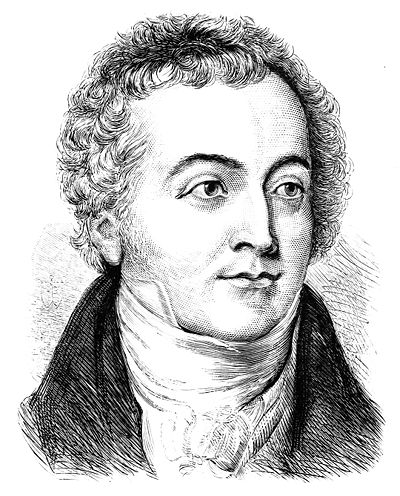
\includegraphics[width=0.7\textwidth]{Bilder/thomas_young.jpg}
    \label{fig:young}
    \caption{Thomas Young (1773-1829) war ein englischer Augenarzt und Physiker und mass als erster die Wellenlängen des Lichts}
\end{marginfigure}

Die wissenschaftliche Notation besteht darin, eine Zahl als Produkt einer Zahl zwischen 1 und 10 und einer Potenz von Zehn aufzuschreiben. Die sogenannte Zehnerpotenz hilft, die Grösse einer Zahl direkt ablesen zu können. 

\begin{margintable}
\begin{tabular}{clc}
\hline
Zehnerpotenz & Name & Abkürzung \\
\midrule
\SI{E12}{} & Tera & T \\
\SI{E9}{} & Giga & G \\
\SI{E6}{} & Mega & M \\
\SI{E3}{} & Kilo & k \\
\SI{E-1}{} & Dezi & d \\
\SI{E-2}{} & Zenti & c \\
\SI{E-3}{} & Milli & m \\
\SI{E-6}{} & Mikro & $\mu$ \\
\SI{E-9}{} & Nano & n \\
\bottomrule
\end{tabular}
\end{margintable}

Achtung: Bei der wissenschaftlichen Notation handelt es sich nicht um eine mathematische Aufgabe, bei der Eingabe eines Wertes wie $6.022 \cdot 10^{23}$ in den Taschenrechner ist also nicht die Multiplikationstaste zu drücken, sondern – je nach Ausführung – die EE- oder EXP-Taste.

\section{(Mass-)Einheiten}
Masseinheiten dienen zum Bestimmen des Wertes physikalischer Grössen. Beim Messen wird die zu messende Grösse mit der Einheit beziehungsweise mit einem Referenzmass 
verglichen, das ein Vielfaches oder ein Teil der Einheit ist. 
Messergebnisse einer Grösse können miteinander nur direkt verglichen werden, wenn sie sich auf die gleiche Einheit beziehen.\footnote{Quelle: \href{http://www.metas.ch}{www.metas.ch}}

Ein Einheitensystem ist ein Satz von Regeln, der die Masseinheiten in Naturwissenschaft und Technik widerspruchsfrei festlegt. Es muss den verschiedensten Anwendungen in 
Wissenschaft, Technik, Handel und Gesellschaft gerecht werden. 
Mit dem wissenschaftlich-technischen Fortschritt muss auch das 
Einheitensystem laufend den neuen Anforderungen angepasst 
werden. 

Das heute weltweit angewandte Einheitensystem, das Internationale Einheitensystem - auch \textbf{SI} genannt nach der französischen Bezeichnung Système international d'unités - ist Ergebnis einer langen geschichtlichen Entwicklung. Das SI wurde 1960\footnote{in der Schweiz 1978} eingeführt und löste in der Folge eine Reihe verschiedener Einheitensysteme ab, die vor allem in den Naturwissenschaften Verwendung 
fanden. Damit wurden komplizierte Umrechnungen überflüssig. Die gesetzlichen Bestimmungen über seine Anwendung sind im Bundesgesetz über das Messwesen und in der Einheiten-Verordnung geregelt. Im SI unterscheidet man die \textbf{Basiseinheiten} und die 
\textbf{abgeleiteten Einheiten}. Die \textbf{7 Basiseinheiten} sind:
\begin{marginfigure}
	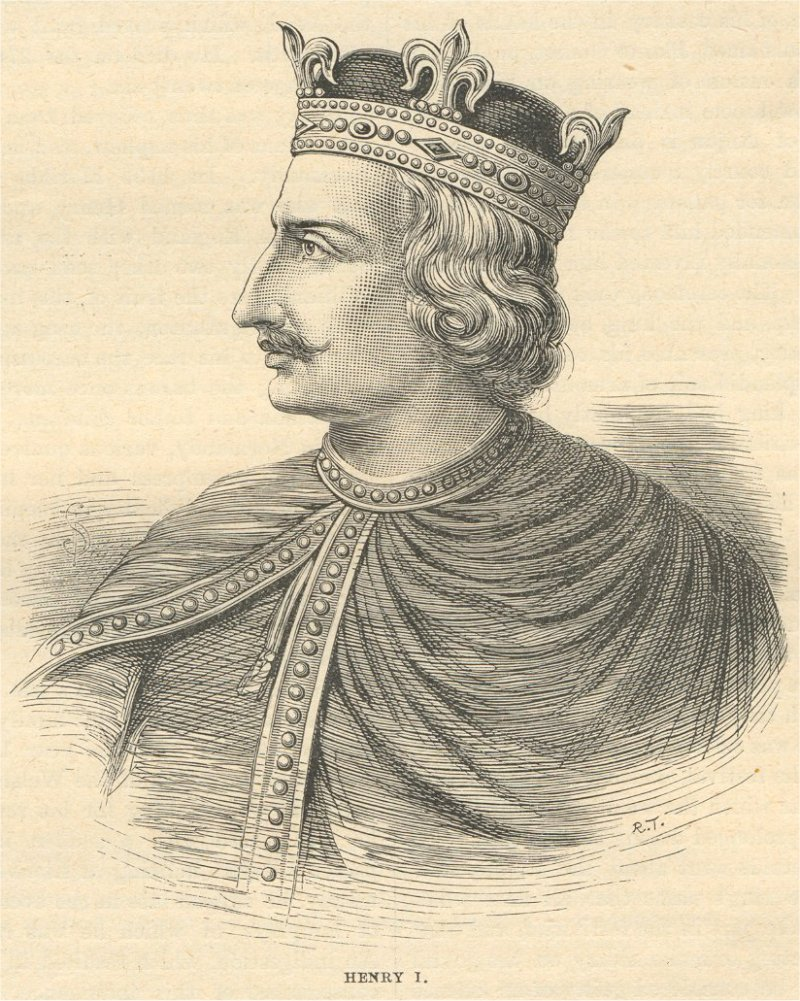
\includegraphics[width=0.7\textwidth]{Bilder/Henry.jpg}
	\caption{König Henry I. von England führte 1011 die Längeneinheit Yard als die Distanz zwischen seiner Nasenspitze und der Daumenspitze seines ausgestreckten Arms ein. Ein Yard entspricht \SI{0.9144}{\metre}}
\end{marginfigure}
\begin{multicols}{2}
\begin{itemize}
	\item \textbf{Kilogramm} (\si{\kilogram}) als Einheit der Masse 
	\item \textbf{Meter} (\si{\metre}) als Einheit der Länge
	\item \textbf{Sekunde} (\si{\second}) als Einheit der Zeit
	\item \textbf{Kelvin} (\si{\kelvin}) als Einheit der Temperatur
	\item \textbf{Ampere} (\si{\ampere}) als Einheit der Stromstärke
	\item \textbf{Candela} (\si{\candela}) als Einheit der Lichtstärke
	\item \textbf{Mol} (\si{mol}) als Einheit der Stoffmenge
\end{itemize} 
\end{multicols}
\begin{figure}
\begin{multicols}{2}
\begin{centering}
\begin{tikzpicture}[scale=0.7]
\def \n {7}
\def \radius {3cm}

\draw[color=gray!50,very thick] circle (3cm);
  \node[draw, circle,minimum width=1 cm,shading=ball,ball color=white] at ({0}:\radius) (s) {\si{\second}};
  \node[draw, circle,minimum width=1 cm,shading=ball,ball color=white] at ({360/\n}:\radius) (K) {\si{\kelvin}};
  \node[draw, circle,minimum width=1 cm,shading=ball,ball color=white] at ({360/\n*2}:\radius) (A) {\si{\ampere}}; 
  \node[draw, circle,minimum width=1 cm,shading=ball,ball color=white] at ({360/\n*3}:\radius) (mol) {\si{\mol}}; 
  \node[draw, circle,minimum width=1 cm,shading=ball,ball color=white] at ({360/\n*4}:\radius) (cd) {\si{\candela}};
  \node[draw, circle,minimum width=1 cm,shading=ball,ball color=white] at ({360/\n*5}:\radius) (kg) {\si{\kilogram}};
  \node[draw, circle,minimum width=1 cm,shading=ball,ball color=white] at ({360/\n*6}:\radius) (m) {\si{\metre}}; 

  \draw[->,>=latex,thick] (s) -- (A);
  \draw[->,>=latex,thick] (s) -- (cd);
  \draw[->,>=latex,thick] (s) -- (m);
  \draw[->,>=latex,thick] (m) -- (A);
  \draw[->,>=latex,thick] (m) -- (cd);
  \draw[->,>=latex,thick] (kg) -- (A);
  \draw[->,>=latex,thick] (kg) -- (cd);
  \draw[->,>=latex,thick] (kg) -- (mol);
\end{tikzpicture}

\begin{tikzpicture}[scale=0.7]
\def \n {7}
\def \radius {3cm}

\draw[color=gray!50,very thick] circle (3cm);
  \node[draw, circle,minimum width=1 cm,shading=ball,ball color=white] at ({0}:\radius) (s) {\si{\second}};
  \node[draw, circle,minimum width=1 cm,shading=ball,ball color=white] at ({360/\n}:\radius) (K) {\si{\kelvin}};
  \node[draw, circle,minimum width=1 cm,shading=ball,ball color=white] at ({360/\n*2}:\radius) (A) {\si{\ampere}}; 
  \node[draw, circle,minimum width=1 cm,shading=ball,ball color=white] at ({360/\n*3}:\radius) (mol) {\si{\mol}}; 
  \node[draw, circle,minimum width=1 cm,shading=ball,ball color=white] at ({360/\n*4}:\radius) (cd) {\si{\candela}};
  \node[draw, circle,minimum width=1 cm,shading=ball,ball color=white] at ({360/\n*5}:\radius) (kg) {\si{\kilogram}};
  \node[draw, circle,minimum width=1 cm,shading=ball,ball color=white] at ({360/\n*6}:\radius) (m) {\si{\metre}}; 

  \draw[->,>=latex,thick] (s) -- (K);
  \draw[->,>=latex,thick] (s) -- (A);
  \draw[->,>=latex,thick] (s) -- (cd);
  \draw[->,>=latex,thick] (s) -- (kg);
  \draw[->,>=latex,thick] (s) -- (m);
  \draw[->,>=latex,thick] (m) -- (K);
  \draw[->,>=latex,thick] (m) -- (cd);
  \draw[->,>=latex,thick] (m) -- (kg);
  \draw[->,>=latex,thick] (kg) -- (cd);
  \draw[->,>=latex,thick] (kg) -- (K);
\end{tikzpicture}
\end{centering}
\end{multicols}

\end{figure}


\subsection{Der Meter} 
\begin{marginfigure}
    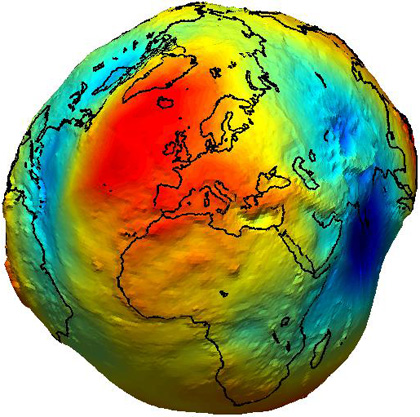
\includegraphics[width=0.7\textwidth]{Bilder/geoid.jpg}
    \label{fig:geoidfig}
    \caption{Die Erde ist unregelmässig geformt und eignet sich nicht als Bezugspunkt. Abweichungen von der Kugelform sind übertrieben dargestellt}
\end{marginfigure}
wurde 1792 durch die Nationalversammlung zu Paris als ein Zehnmillionstel der Entfernung zwischen Nordpol und Äquator definiert. Später kommt aus, dass dieser Meter durch einen Fehler um \SI{0.2}{\milli \metre} zu kurz geraten ist. Die Idee, den Meter durch mit Hilfe der Erde zu definieren ist jedoch nicht wirklich nützlich, denn die Erde besitzt keine regelmässige Form und ist Veränderungen unterworfen. Heute ist der Meter durch die konstante Lichtgeschwindigkeit im Vakuum definiert.
\begin{definition}\index{Meter!Definition}
Länge der Strecke, die das Licht im Vakuum während der Dauer von $\frac{1}{299792458}\si{\second}$ zurücklegt.
\end{definition}

\subsection{Das Kilogramm} 
\begin{marginfigure}
    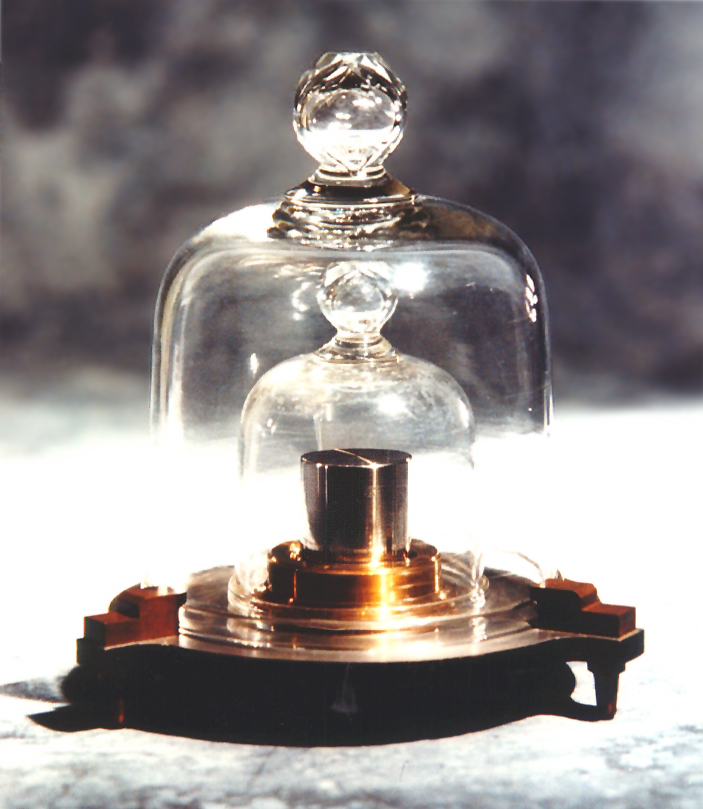
\includegraphics[width=0.7\textwidth]{Bilder/urkilogram.jpg}
    \label{fig:urkilogramfig}
    \caption{Der nationale Kilogramm-Prototyp von Dänemark, eine der über 80 Kopien des Urkilograms}
\end{marginfigure}
ist die Einheit der Masse.  Masse ist das Mass der Menge einer Substanz. Ein Kilogramm entspricht exakt der Masse des Urkilogrammes in Paris, eines Zylinders aus einer Platin-Iridium Legierung. Kopien des Originals werden immer wieder mit dem Urkilogramm verglichen. Diese Definition ist nicht wirklich sehr verlässlich und es werden Wege gesucht, auch das Kilogramm an eine Naturkonstante zu knüpfen, so wie dies bei den anderen 6 SI-Einheiten gemacht wurde.
\begin{definition}\index{Kilogramm!Definition}
Das Kilogramm ist gleich der Masse des Internationalen Kilogrammprototyps.
\end{definition}

\subsection{Die Sekunde} wurde bis in die 1930er Jahre über die Tageslänge definiert. Dann stellte man fest, dass diese Zeitdauer nicht konstant ist\footnote{die Tageslänge wird beeinflusst durch den Mond, abschmelzende Gletscher und sogar durch Winde} und über längere Zeiträume sogar abnimmt. Heute wird sie durch die Eigenschaften von Atomen definiert: Sie wird definiert durch die Eigenschaft der von bestimmten Atomen ausgesendeten Strahlung. Diese neue Definition ist an eine Naturkonstante geknüpft und wird sich somit zeitlich nicht mehr verändern.
\begin{definition}\index{Sekunde!Definition}
Das \SI{9192631770}{}-fache der Periodendauer der dem Übergang zwischen den beiden Hyperfeinstrukturniveaus des Grundzustandes von Atomen des Caesium-Isotops 133Cs entsprechenden Strahlung.
\end{definition}
\begin{marginfigure}
    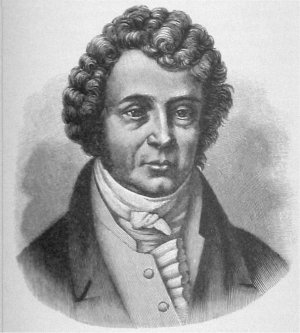
\includegraphics[width=0.7\textwidth]{Bilder/ampere.jpg}
    \label{fig:amperefig}
    \caption{André-Marie Ampère (1775-1836) war ein französischer Physiker und Mathematiker. Nach ihm ist die internationale Einheit der Stromstärke Ampere benannt.}
\end{marginfigure}
\subsection{Das Ampere}
ist die Einheit der Stromstärke. Sie wird über eine Kraftwirkung definiert.
\begin{definition}\index{Ampere!Definition}
Stärke eines konstanten elektrischen Stromes, der, durch zwei parallele, geradlinige, unendlich lange und im Vakuum im Abstand von 1 Meter voneinander angeordnete Leiter von vernachlässigbar kleinem, kreisförmigem Querschnitt fliessend, zwischen diesen Leitern pro Meter Leiterlänge die Kraft \SI{2E-7}{} Newton hervorrufen würde
\end{definition}

\subsection{Das Kelvin}
ist die Einheit der thermodynamischen Temperatur. Das Kelvin wird über eine Eigenschaft des Wassers definiert. In der Physik wird die Kelvinskala der Celsiusskala vorgezogen, da sie auf dem absoluten Nullpunkt basiert. Es gibt somit keine negativen Temeraturen in der Einheit Kelvin!
\begin{marginfigure}
    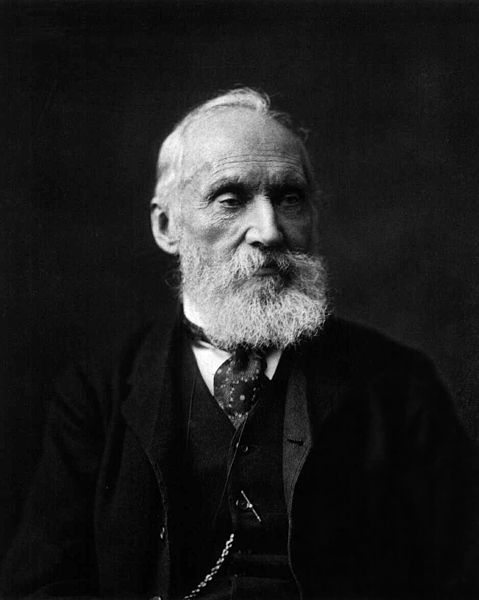
\includegraphics[width=0.7\textwidth]{Bilder/kelvin.jpg}
    \label{fig:kelvinfig}
    \caption{William Thomson, 1. Baron Kelvin, meist als Lord Kelvin bezeichnet, (1824-1907) war ein in Irland geborener britischer Physiker.}
\end{marginfigure}
\begin{definition}\index{Kelvin!Definition}
$1/273.16$ der thermodynamischen Temperatur des Tripelpunkts von Wasser genau definierter isotopischer Zusammensetzung.
\end{definition}

\subsection{Das Mol} ist die Einheit der Stoffmenge (Substanzmenge). Es wird über die Anzahl Atome eines Bestimmten Elementes definiert.  Bei Benutzung des Mol müssen die Einzelteilchen spezifiziert sein und können Atome, Moleküle, Ionen, Elektronen sowie andere Teilchen oder Gruppen solcher Teilchen genau angegebener Zusammensetzung sein.
\begin{definition}\index{Mol!Definition}
Die Stoffmenge eines Systems, das aus ebenso viel Einzelteilchen besteht, wie Atome in 12 Gramm des Kohlenstoff-Isotops 12C in ungebundenem Zustand enthalten sind.
\end{definition}

\subsection{Die Candela} ist die Einheit der Lichtstärke. Sie wird über die Strahlung einer bestimmten Frequenz und Leistung definiert.
\begin{definition}\index{Candela!Definition}
Die Lichtstärke in einer bestimmten Richtung einer Strahlungsquelle, die monochromatische Strahlung der Frequenz \SI{540E12}{} Hertz aussendet und deren Strahlstärke in dieser Richtung $\frac{1}{683}$ Watt pro Steradiant beträgt.
\end{definition}

\begin{margintable}
\begin{tabular}{l l l}
	\toprule
	phys. Grösse  & Abkürzung  & Einheit \\
	\midrule
	Masse	& $m$	     & \si{\kilogram} \\
	Länge 	& $l$	     & \si{\metre} \\
	Zeit	& $t$  	     & \si{\second} \\
	Temperatur & $T$     & \si{\kelvin} \\
	Stromstärke & $I$    & \si{\ampere} \\
	Lichtstärke & $l$    & \si{\candela} \\
	Stoffmenge & $N$     & \si{mol} \\
	\bottomrule
\end{tabular}
\caption{Die SI-Basiseinheiten}
\end{margintable}

\subsection{Unabhängigkeit von Raum und Zeit}
Eine wichtige Forderung an die Basiseinheiten ist ihre \textbf{Unabhängigkeit von Raum und Zeit}: Die Basiseinheiten sollten 
jederzeit in irgend einem Labor reproduziert werden können. 
Zur Erfüllung dieser Forderung wurden ihre Definitionen schon 
mehrmals geändert. Sie basieren heute, mit Ausnahme des 
Kilogramms, nicht mehr auf Massverkörperungen (Vergleichen mit einem Urmass), sondern auf 
konstanten Eigenschaften der Natur, die in besonderen Experimenten jederzeit und überall gemessen werden können. Da die Definitionen einiger Einheiten noch nicht von Naturkonstanten abhängig sind (insbesondere die Definition des Kilogrammes), werden diese in Zukunft noch abgeändert werden.
\subsection{Abgeleitete Einheiten}
Die \textbf{abgeleiteten} werden aus den Basiseinheiten durch die gleichen algebraischen Beziehungen gebildet, wie sie aufgrund der Naturgesetze für die entsprechenden Grössen gelten. 
Ein wichtiger Gesichtspunkt ist dabei die Kohärenz, das heisst 
die Eigenschaft, abgeleitete Einheiten durch Multiplikation und 
Division von Basiseinheiten zu bilden, ohne weitere Zahlenfaktoren zu verwenden. Diese Abgeleiteten Einheiten werden dann \textbf{Grundeinheiten} genannt.

\begin{example}
Die Dichte eines Objektes berechnet sich aus Masse geteilt durch Volumen. Die Einheit der Masse ist das Kilogramm (SI-Basiseinheit) und die Einheit des Volumens ist der Kubikmeter (Abgeleitet von der SI-Basiseinheit Meter). Die Einheit der Dichte ist also: \si{\kilogram \per \metre \cubed}. Dies ist die Grundeinheit der Dichte.
\end{example}
\subsection{SI-fremde Einheiten}
Neben den SI-Einheiten ist es aus praktischen Gründen oft noch üblich inkohärent abgeleitete Einheiten, oder SI-fremde Einheiten zu benutzen. In diesen Fällen ist es dann wichtig die Umrechnungsfaktoren in das SI zu kennen. 
\begin{example}
Die Minute ($\SI{1}{\minute} = \SI{60}{\second}$)
\end{example}

%https://docs.google.com/file/d/0B4nWIuz6_aEMS0ZmbVI4WHdTLXFFMURob0V1M21Odw/edit

\section{Physikalische Grössen}
Die physikalischen Grössen spielen eine besonders wichtige Rolle in der Physik. Was ist jedoch eine physikalische Grösse? 

\begin{definition}\index{physikalische Grösse!Definition} %Messbare Eigenschaften von Objekten
physikalische Grösse
    \vspace{2cm}
\end{definition}
\begin{example}
Das Volumen $V$ gibt an, wie viel Raum ein Körper einnimmt, die Masse $m$ gibt an, wie schwer und träge ein Körper ist.
\end{example}
Wir unterscheiden ungerichtete und gerichtete physikalische Grössen. Zu den ungerichteten Grössen\footnote{Fachbegriff Skalar} gehören zum Beispiel die Temperatur oder die Masse. Beispiele für gerichtete Grössen\footnote{Fachbegriff Vektor} sind die Geschwindigkeit oder die Kraft.

Da physikalische Grössen messbar sind, kann man dementsprechend einen Grössenwert angeben. Der Grössenwert besteht immer aus:
\[ \text{Grössenwert} = \text{Zahlenwert} \cdot \text{Einheit} \]
\begin{example}
Die Dichte von Gold beträgt 19302 Kilogramm pro Kubikmeter, also:
\[ \rho_{Gold} = \SI{19302}{\kilo \gram \per \metre \cubed} \]
\end{example}

\section{Abweichungen und Ungenauigkeiten - oder wie runde ich?} \marginnote{Ein wichtiges Kriterium zur Unterscheidung oder Bewertung von systematischen und statistischen Fehlern ist die Richtung der Abweichungen: Systematische Fehler sind einseitig gerichtet und bei wiederholten Messungen unter identischen Bedingungen immer gleich, statistische Fehler dagegen schwanken im Vorzeichen und Betrag um einen Mittelwert.}
Alle Messungen sind von Natur aus mit Fehlern behaftet. Dabei ist hier nicht von systematischen Fehlen die Rede, z.B. weil ein Messgerät falsch justiert oder Meswerte falsch abgelesen werden, sondern von statistischen Fehlern.

Da das Rechnen mit fehlerbehafteten Grössen zu enormen Abweichungen führen kann – bei Ergebnissen aber nicht selten exzessiv Nachkommastellen angegeben werden, die eine falsche Genauigkeit vortäuschen – gilt daher für alle Berechnungen im Physik-Unterricht folgende Regeln: %https://www.evernote.com/shard/s22/res/c9b06e8e-2924-4f8a-be77-0ad8241d3357/nga_aef.pdf?search=signifikant
\begin{regel}
Runden
\vspace{6cm}
\end{regel}

\begin{example}
Ein Schüler misst, dass ein Stein mit einem Volumen von \SI{251}{\centi \metre \cubed} eine Masse von \SI{591.9}{\gram} besitzt. Daraus ermittelt die Dichte $\rho$:
\[ \rho = \frac{\SI{591.9}{\gram}}{\SI{251}{\centi \metre \cubed}} = \SI{2.358167331}{\gram \per \centi \metre \cubed} \]

Da jedoch beide Messungen eine begrenzte Genauigkeit besitzen, macht eine solche Angabe keinen Sinn. Mit der Regel für das Runden betrachten wir nun die Zahl mit der kleinsten Anzahl signifikanter Stellen, dies ist $251$ (3 signifikante Stellen). Das Resultat wird also auch auf 3 signifikante Stellen gerundet:
\[ \rho = \frac{\SI{591.9}{\gram}}{\SI{251}{\centi \metre \cubed}} = \SI{2.36}{\gram \per \centi \metre \cubed} \]
\end{example}

\subsection{Signifikante Stellen}
Als signifikante Stellen versteht man alle Stellen einer Zahl von der ersten von null verschiedenen Stelle von vorn bis zur Rundungsstelle. Dies ist die letzte Stelle, die nach dem Runden noch angegeben werden kann. 

\begin{example}

\begin{tabular}{clc}

Messwert & Anzahl signifikanter Stellen \\
\midrule
\SI{12}{m} & 2 signifikante Stellen (die Messung ist metergenau) \\
\SI{25.38}{m} & 4 signifikante Stellen (die Messung ist zentimetergenau)  \\
\SI{125.005}{m} & 6 signifikante Stellen (die Messung ist millimetergenau) \\
\SI{0.000305}{m} & 3 signifikante Stellen (die Messung ist mikrometergenau) \\
\SI{3.2500}{} & 5 signifikante Stellen \\
\SI{2000}{m} & Ungeklärt, 1 bis 4 signifikante Stellen. Man könnte aufklären \\
 & indem man schreibt: \\
 & 2 km (1 signifikante Stelle) \\
 & 2,0 km (2 signifikante Stellen) \\ 
 & 2,00 km (4 signifikante Stellen) \\
 & 2,000 km (4 signifikante Stellen)  \\


\end{tabular}
\end{example}
